\section{SYSTEM MODEL}
\label{sec: system_model}


\begin{frame}{}
    以下では, 上記の説明から抽出したマルチスレッドエグゼキュータのリアルタイム関連の動作をカバーするスケジューリングモデルを紹介する
\end{frame}

\begin{frame}{}
\assume{簡単にするために, wait\_set にアクセスまたは更新するスレッドによって発生するオーバヘッドはゼロであると仮定する}
\end{frame}

\begin{frame}{Notations1}
    \begin{table}[tb]
        \adjustbox{max width=\textwidth}{
            \centering\begin{tabular}{|c|l|} \hline
                \textbf{Notations}      & \textbf{Descriptions}                                                                         \\\hline
                $C_i$                   & チェイン                                                                                      \\\hline
                $m$                     & スレッド数                                                                                    \\\hline
                $\Gamma $               & チェインのセット                                                                              \\\hline
                $c_{i,j}$               & $C_i$の$j$番目のコールバック                                                                  \\\hline
                $e_{i,j}$               & $c_{i,j}$のWCET                                                                               \\\hline
                $E_i$                   & $C_i$内のコールバックのWCETの合計                                                             \\\hline
                $D_i$                   & $C_i$のデッドライン                                                                           \\\hline
                $T_i$                   & $C_i$の周期                                                                                   \\\hline
                $U_i$                   & $C_i$の利用率                                                                                 \\\hline
                $\mathcal{G}(c_{i,j}) $ & $c_{i,j}$が属すmutually exclusiveコールバックグループのインデックス                           \\\hline
                $\theta_i$              & \tabml{$\mathcal{C}_{i}$ の各コールバックが属すmutually exclusiveコールバックグループの集合 \\ $\theta_{i}=\cup_{\forall c_{i, j} \in \mathcal{C}_{i}}\left\{\mathcal{G}\left(c_{i, j}\right)\right\}$} \\\hline
            \end{tabular}
        }
    \end{table}
\end{frame}

\begin{frame}{Notation2}
    \begin{table}[tb]
        \adjustbox{max width=\textwidth}{
            \centering\begin{tabular}{|c|l|} \hline
                \textbf{Notations} & \textbf{Descriptions}                                       \\\hline
                $J_{i}^{k}$        & $\mathcal{C}_{i}$ の $k$番目のインスタンス                  \\\hline
                $c_{i, j}^{k}$     & $J_{i}^{k}$ に含まれる$c_{i, j}$ のコールバックインスタンス \\\hline
            \end{tabular}
        }
    \end{table}
\end{frame}

\subsection{Workload Model}
\label{ssec: workload_model}

\begin{frame}{チェーンの定義}

    \begin{itemize}
        \item $m$ スレッド上のマルチスレッドエグゼキュータによってスケジュールされた一連の独立した処理チェーン (略してチェーンと呼ぶ) $\Gamma=\left\{\mathcal{C}_{1}, \mathcal{C}_{2}, \cdots, \mathcal{C}_{|\Gamma|}\right\}$ を検討する

        \assume{各スレッドは専用プロセッサに静的に展開されており,スレッドはいつでもプロセッサを使用できる}

        \item 各チェーン $\mathcal{C}_{i} \in \Gamma$ は, コールバック $\mathcal{C}_{i}=\left\{c_{i, 1}, c_{i, 2}, \cdots, c_{i,\left|\mathcal{C}_{i}\right|}\right\}$ の順序付けられたシーケンスで構成される
        \item $\mathcal{C}_{i}$ の最初のコールバック $c_{i, 1}$ (それぞれ, 最後のコールバック $c_{i,\left|\mathcal{C}_{i}\right|}$ ) は, $\mathcal{C}_{i}$ のソースコールバック (それぞれ, シンクコールバック) と呼ばれる
    \end{itemize}
\end{frame}

\begin{frame}{}
    \begin{itemize}
        \item 各コールバック $c_{i, j}$ は最悪実行時間 (WCET) $e_{i, j}$ によって特徴付けられる
        \item コールバックは, 固有のmutually exclusive コールバックグループまたはreentrant コールバックグループのいずれかに属している
    \end{itemize}
\end{frame}

\begin{frame}{}
    \begin{itemize}
        \item チェーン $\mathcal{C}_{i}$ は, チェーンインスタンスの無限シーケンスをリリースする
        \item $T_{i}$ の周期は, $\mathcal{C}_{i} \cdot \mathcal{C}_{i}$ の 2 つの連続するチェーンインスタンスのリリース時刻の間の最小間隔
        \item 相対デッドライン $D_{i}$ があり, 時間 $r$ でリリースされた $\mathcal{C}_{i}$ の各チェーンインスタンスは, その絶対デッドライン $r+D_{i}$ までに終了する必要がある
        \item チェーンには制約付きデッドライン, つまり $D_{i} \leq T_{i}$ があると想定している
        \item $\mathcal{C}_{i}$ の利用率は $U_{i}=E_{i} / T_{i}$ である
    \end{itemize}
\end{frame}

\begin{frame}{}
    \begin{itemize}
        \item $J_{i}^{k}$ 内の連続する要素 $c_{i, j}^{k}$ と $c_{i, j+1}^{k}$ の各ペアについて, $c_{i, j}^{k}$ を $c_{i, j+1}^{k}$ の先行要素, $c_{i, j+1}^{k}$ を $c_{i, j}^{k}$ の後続要素と呼ぶ
        \item 非シンクコールバックインスタンス $c_{i, j}^{k}$ が実行を終了すると, 後続のインスタンスを呼び出すメッセージが生成される
    \end{itemize}
\end{frame}

\begin{frame}{応答時間の定義}
    \begin{itemize}
        \item 応答時間 $R\left(J_{i}^{k}\right)$ は,  $J_{i}^{k}$ のリリース時刻と終了時間の間の時間間隔である
        \item チェーン $\mathcal{C}_{i}$ の最悪応答時間 $\mathcal{R}_{i}^{w c}$ は, そのすべてのインスタンスの中で最大の応答時間である
        \item チェーンは, そのすべてのインスタンスがデッドラインを満たしている場合 (つまり, $\mathcal{R}_{i}^{w c} \leq D_{i}$), スケジュール可能であると言われ, $\Gamma$ は, すべてのチェーンがスケジュール可能である場合 (つまり, $\forall i: \mathcal{R}_{i}^{w c} \leq D_{i}$), スケジュール可能であると呼ぶ
    \end{itemize}
\end{frame}

\begin{frame}{本論文の目的}
    この論文の目的は, システム $\Gamma$ がマルチスレッドエグゼキュータでスケジュール可能かどうかを判断し, $\Gamma$ がスケジュール可能である場合, 各チェーン $\mathcal{C}_{i} \in \Gamma$ の $\mathcal{R}_{i}^{w c}$ の安全な上界を計算することである
\end{frame}


\subsection{Scheduling Model}
\label{ssec: scheduling_model}


\begin{frame}{}
    \begin{itemize}
        \item 実行時に, $J_{i}^{k}$ 内の最初のコールバックインスタンス $c_{i, 1}^{k}$ は, $J_{i}^{k}$ がリリースされるときにリリースされる
        \item $J_{i}^{k}$ 内の別のコールバックインスタンスは, その先行の終了時, つまり, 先行からの入力メッセージが利用可能になった時点でリリースされる
        \item 同じコールバックの複数のインスタンスがリリースされた場合、リリース時刻を基準にFIFOにエンキューされる
    \end{itemize}
\end{frame}

\begin{frame}{Pending}


    \begin{itemize}
        \item コールバックインスタンス$c_{i, j}$は、それがリリースされ、その前のインスタンスがすべて実行中か終了しているとき、\al{pending} と呼ぶ
        \item pendingコールバックインスタンス$c_{i, j}$は、\al{ready} または\al{P-blocked} のいずれかである
              \begin{itemize}
                  \item  $c_{i, j}$ がmutually exclusive コールバックグループに属している場合, $c_{i, j}$ と同じコールバックグループ内のコールバックのインスタンス ($c_{i, j}$ 自体を含む) が実行されていない場合, $c_{i, j}$ はreadyである
                  \item それ以外の場合, $c_{i, j}$ は P-blockedされる

                  \item  $c_{i, j}$ が再入可能コールバックグループに属している場合, pending $c_{i, j}$ は常に ready である
              \end{itemize}
    \end{itemize}
\end{frame}

\begin{frame}{$\Omega$}
    エグゼキュータは, 実行のために選択できるreadyコールバックインスタンスを記録するreadyセット $\Omega$ を持っている
\end{frame}

\begin{frame}{Eligible}
    \begin{itemize}
        \item $\Omega$ 内の ready のコールバックインスタンス $c_{i, j}$ が選択されるための前提条件は, \al{eligible} であることである
        \item mutually exclusive コールバックグループに属す $\Omega$ 内のコールバックインスタンス $c_{i, j}$ は, $c_{i, j}$ と同じコールバックグループ内のコールバックのインスタンスが実行されていない場合に eligible であり, それ以外の場合は \al{R-blocked} される
        \item 対照的に, reentrant コールバックグループに属すコールバックインスタンスは, $\Omega$ にある場合は常に eligible である
        \item つまり, いつでも, $\Omega$ のコールバックインスタンスは eligible であるか, R-blockedされている
        \item つまり, mutually exclusive同じコールバックグループ内のコールバックのコールバックインスタンスは, 並列に実行されることは決してない
    \end{itemize}
\end{frame}

\begin{frame}{updated, poling point}
    \begin{itemize}
        \item コールバックインスタンスは, ready でもすぐには $\Omega$ に追加されない
        \item 代わりに, $\Omega$ に eligible なコールバックがなく, スレッドがアイドル状態の場合にのみ, ready のコールバックインスタンスを $\Omega$ に追加できる
        \item $\Omega$ は, $\Omega$ に新しい要素が追加された時点で更新されると言う
        \item さらに, $\Omega$ が更新されると, まず $\Omega$ が $\emptyset$ に設定され, その後, 現在すべての ready コールバックインスタンスが $\Omega$ に追加される
        \item 特に, $\Omega$ が更新される時点を\al{ポーリングポイント}として定義する
        \item 一連のコールバックインスタンスが同じポーリングポイントで $\Omega$ に追加された場合, これらのインスタンスは同じバッチにあると言う
    \end{itemize}
\end{frame}

\begin{frame}{}
    \begin{itemize}
        \item $\Omega$ 内のeligibleなコールバックインスタンスは、$m$ 個のスレッドによって1つずつ選択され、ノンプリエンプティブに実行される
        \item スレッドとは、処理リソースの観点から、対応するプロセッサを表すものである
    \end{itemize}
\end{frame}

\begin{frame}{}
    \begin{itemize}
        \item eligibleなコールバックインスタンスを選択する順序は, それらの優先度によって異なる
        \item 各コールバックには固定の固有の優先度があり, そのすべてのインスタンスがこの優先度を継承する
        \item $h p\left(c_{i, j}\right)$ を使用して, コールバック $c_{i, j}$ よりも優先度の高い一連のコールバックを示す
        \item 実行するコールバックインスタンスが選択されると, $\Omega  c_{i, j}$ から削除される
    \end{itemize}
\end{frame}

\begin{frame}{}
    \begin{itemize}
        \item $c_{i, j}$ が P-blockedまたは R-blockedのいずれかである場合, \al{ブロックされている}と呼ぶ
        \item $J_{i}^{k}$ のコールバックインスタンスが実行されているときにチェーンインスタンス $J_{i}^{k}$ が実行されており, $J_{i}^{k}$ のコールバックインスタンスがブロックされているときに \al{$J_{i}^{k}$ がブロックされている}と言う
        \item スレッドは, 何らかのコールバックインスタンスが実行されているときは\al{ビジーである}と呼び, コールバックインスタンスが実行されていないときは\al{アイドル状態}と呼ぶ
    \end{itemize}
\end{frame}

\begin{frame}{例}
    \begin{itemize}
        \item $\mathcal{C}_{1}=\left\{c_{1,1}, c_{1,2}\right\}, \mathcal{C}_{2}=\left\{c_{2,1}, c_{2,2}\right\}$ と $\mathcal{C}_{3}=\left\{c_{3,1}, c_{3,2}, c_{3,3}, c_{3,4}\right\}$ の 2 つのスレッドでスケジュールされた 3 つのチェーンがある
        \item 特に, $c_{2,2}$ と $c_{3,2}$ はmutually exclusive同じコールバックグループに属し, 他のコールバックはreentrant コールバックグループに属す
        \item すべてのコールバックの優先度と WCET を図 3(b) に示す
        \item 数字が小さいほど優先度が高くなる

    \end{itemize}
    \centering
    \adjustbox{max width=\textwidth, max height=0.35\textheight}{
        \includegraphics{figure/system_model_example_a_b.png}
    }
\end{frame}


\begin{frame}{}
    \begin{itemize}
        \item 上矢印は, チェーンインスタンスのリリース時刻を表す
        \item 右の表は各ポーリングポイントでの $\Omega$ のコールバックインスタンスを示す
    \end{itemize}
    \centering
    \adjustbox{max width=\textwidth, max height=0.6\textheight}{
        \includegraphics{figure/system_model_example_c_d.png}
    }
\end{frame}

\begin{frame}{R-blocked 例}
    \vspace{\headerheight}
    \centering
    \adjustbox{max width=\textwidth, max height=0.7\textwidth}{
        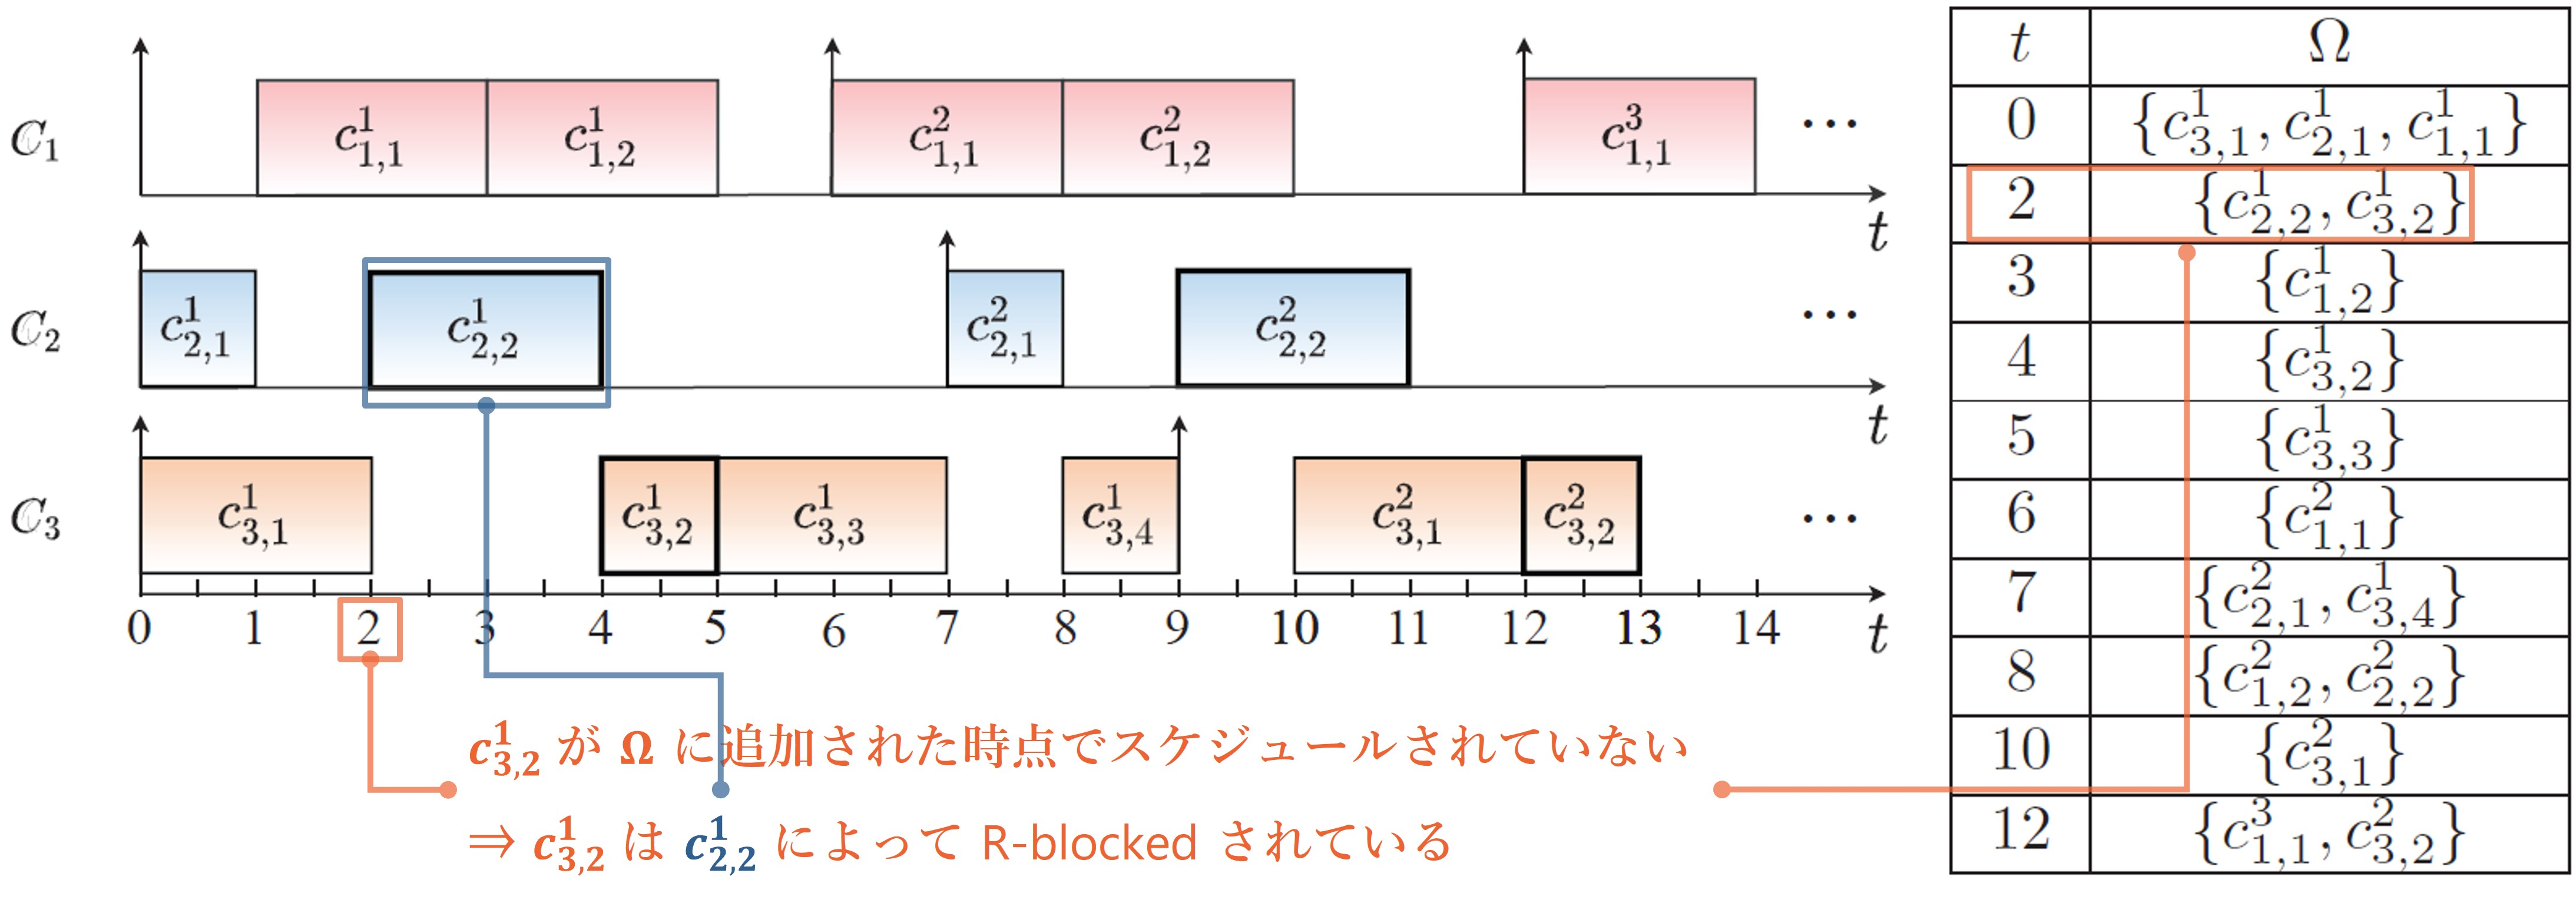
\includegraphics{figure/system_model_example_sup1.jpg}
    }
\end{frame}

\begin{frame}{}
    \begin{itemize}
        \item $c_{2,2}^{1}$ によって R-block される $c_{3,2}^{1}$ は eligible でないため, $\Omega$ から削除される
        \item $c_{3,2}^{1}$ が $\Omega$ から削除された後, $(2,4)$ の時間間隔中に P-blocked され, $\Omega$ に追加できない
    \end{itemize}
\end{frame}
